\documentclass[tikz,border=8pt]{standalone}
\usepackage{amsmath}
\usetikzlibrary{arrows.meta}
\definecolor{ink}{HTML}{21352F}\definecolor{teal}{HTML}{087F7B}
\definecolor{blue}{HTML}{4B77A8}\definecolor{gold}{HTML}{C58B2A}\definecolor{rose}{HTML}{B65A62}
\begin{document}
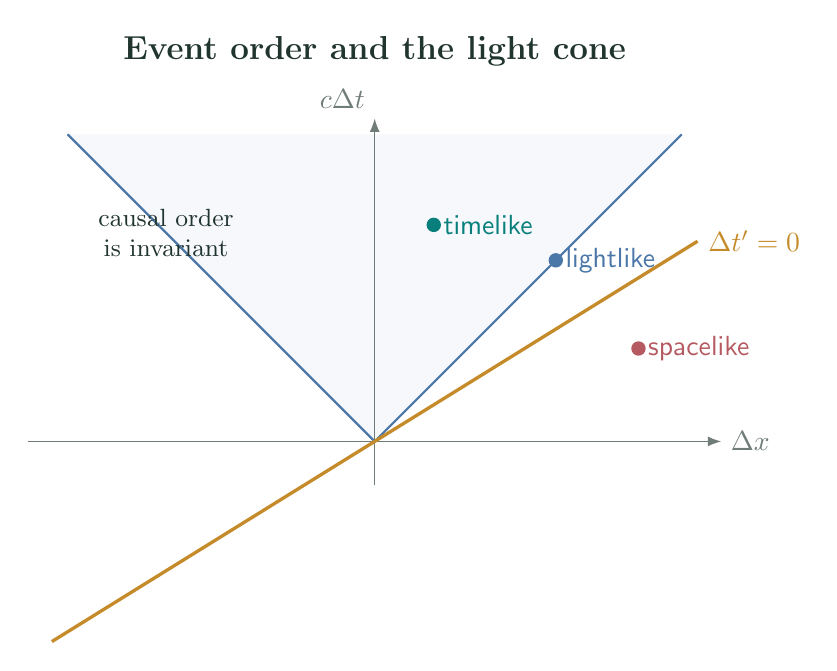
\begin{tikzpicture}[font=\sffamily,text=ink,>=Latex]
  \def\bet{0.62}
  \node[font=\bfseries\large] at (0,4.95) {Event order and the light cone};
  \fill[blue!5] (0,0)--(-3.9,3.9)--(3.9,3.9)--cycle;
  \draw[->,ink!65] (-4.4,0)--(4.4,0) node[right] {$\Delta x$};
  \draw[->,ink!65] (0,-.55)--(0,4.1) node[above left] {$c\Delta t$};
  \draw[blue,thick] (-3.9,3.9)--(0,0)--(3.9,3.9);
  \draw[gold,very thick] (-4.1,{-4.1*\bet})--(4.1,{4.1*\bet}) node[right] {$\Delta t'=0$};
  \fill[teal] (.75,2.75) circle (2.6pt) node[right] {timelike};
  \fill[blue] (2.3,2.3) circle (2.6pt) node[right] {lightlike};
  \fill[rose] (3.35,1.18) circle (2.6pt) node[right] {spacelike};
  \node[font=\small,align=center] at (-2.65,2.65) {causal order\\is invariant};
\end{tikzpicture}
\end{document}
